\documentclass[a4paper, 12pt]{report}
\usepackage{graphicx}
\usepackage[backend=biber,style=alphabetic,sorting=ynt]{biblatex}
\usepackage{blindtext}
\usepackage{hyperref}
\usepackage{xurl}
\usepackage{amsmath}
\usepackage{bm}
\addbibresource{citations.bib}

\begin{document}
\begin{titlepage}
    \begin{center}
        \vspace*{1cm}

        \Large{
            \textbf{matsubara}
        
            \textbf{Case-based Recommendation for \\ Music Playlists}
        
            \vspace{0.5cm}
        
            \textit{Alexander Stradnic}
        
            \vspace{3cm}
        
            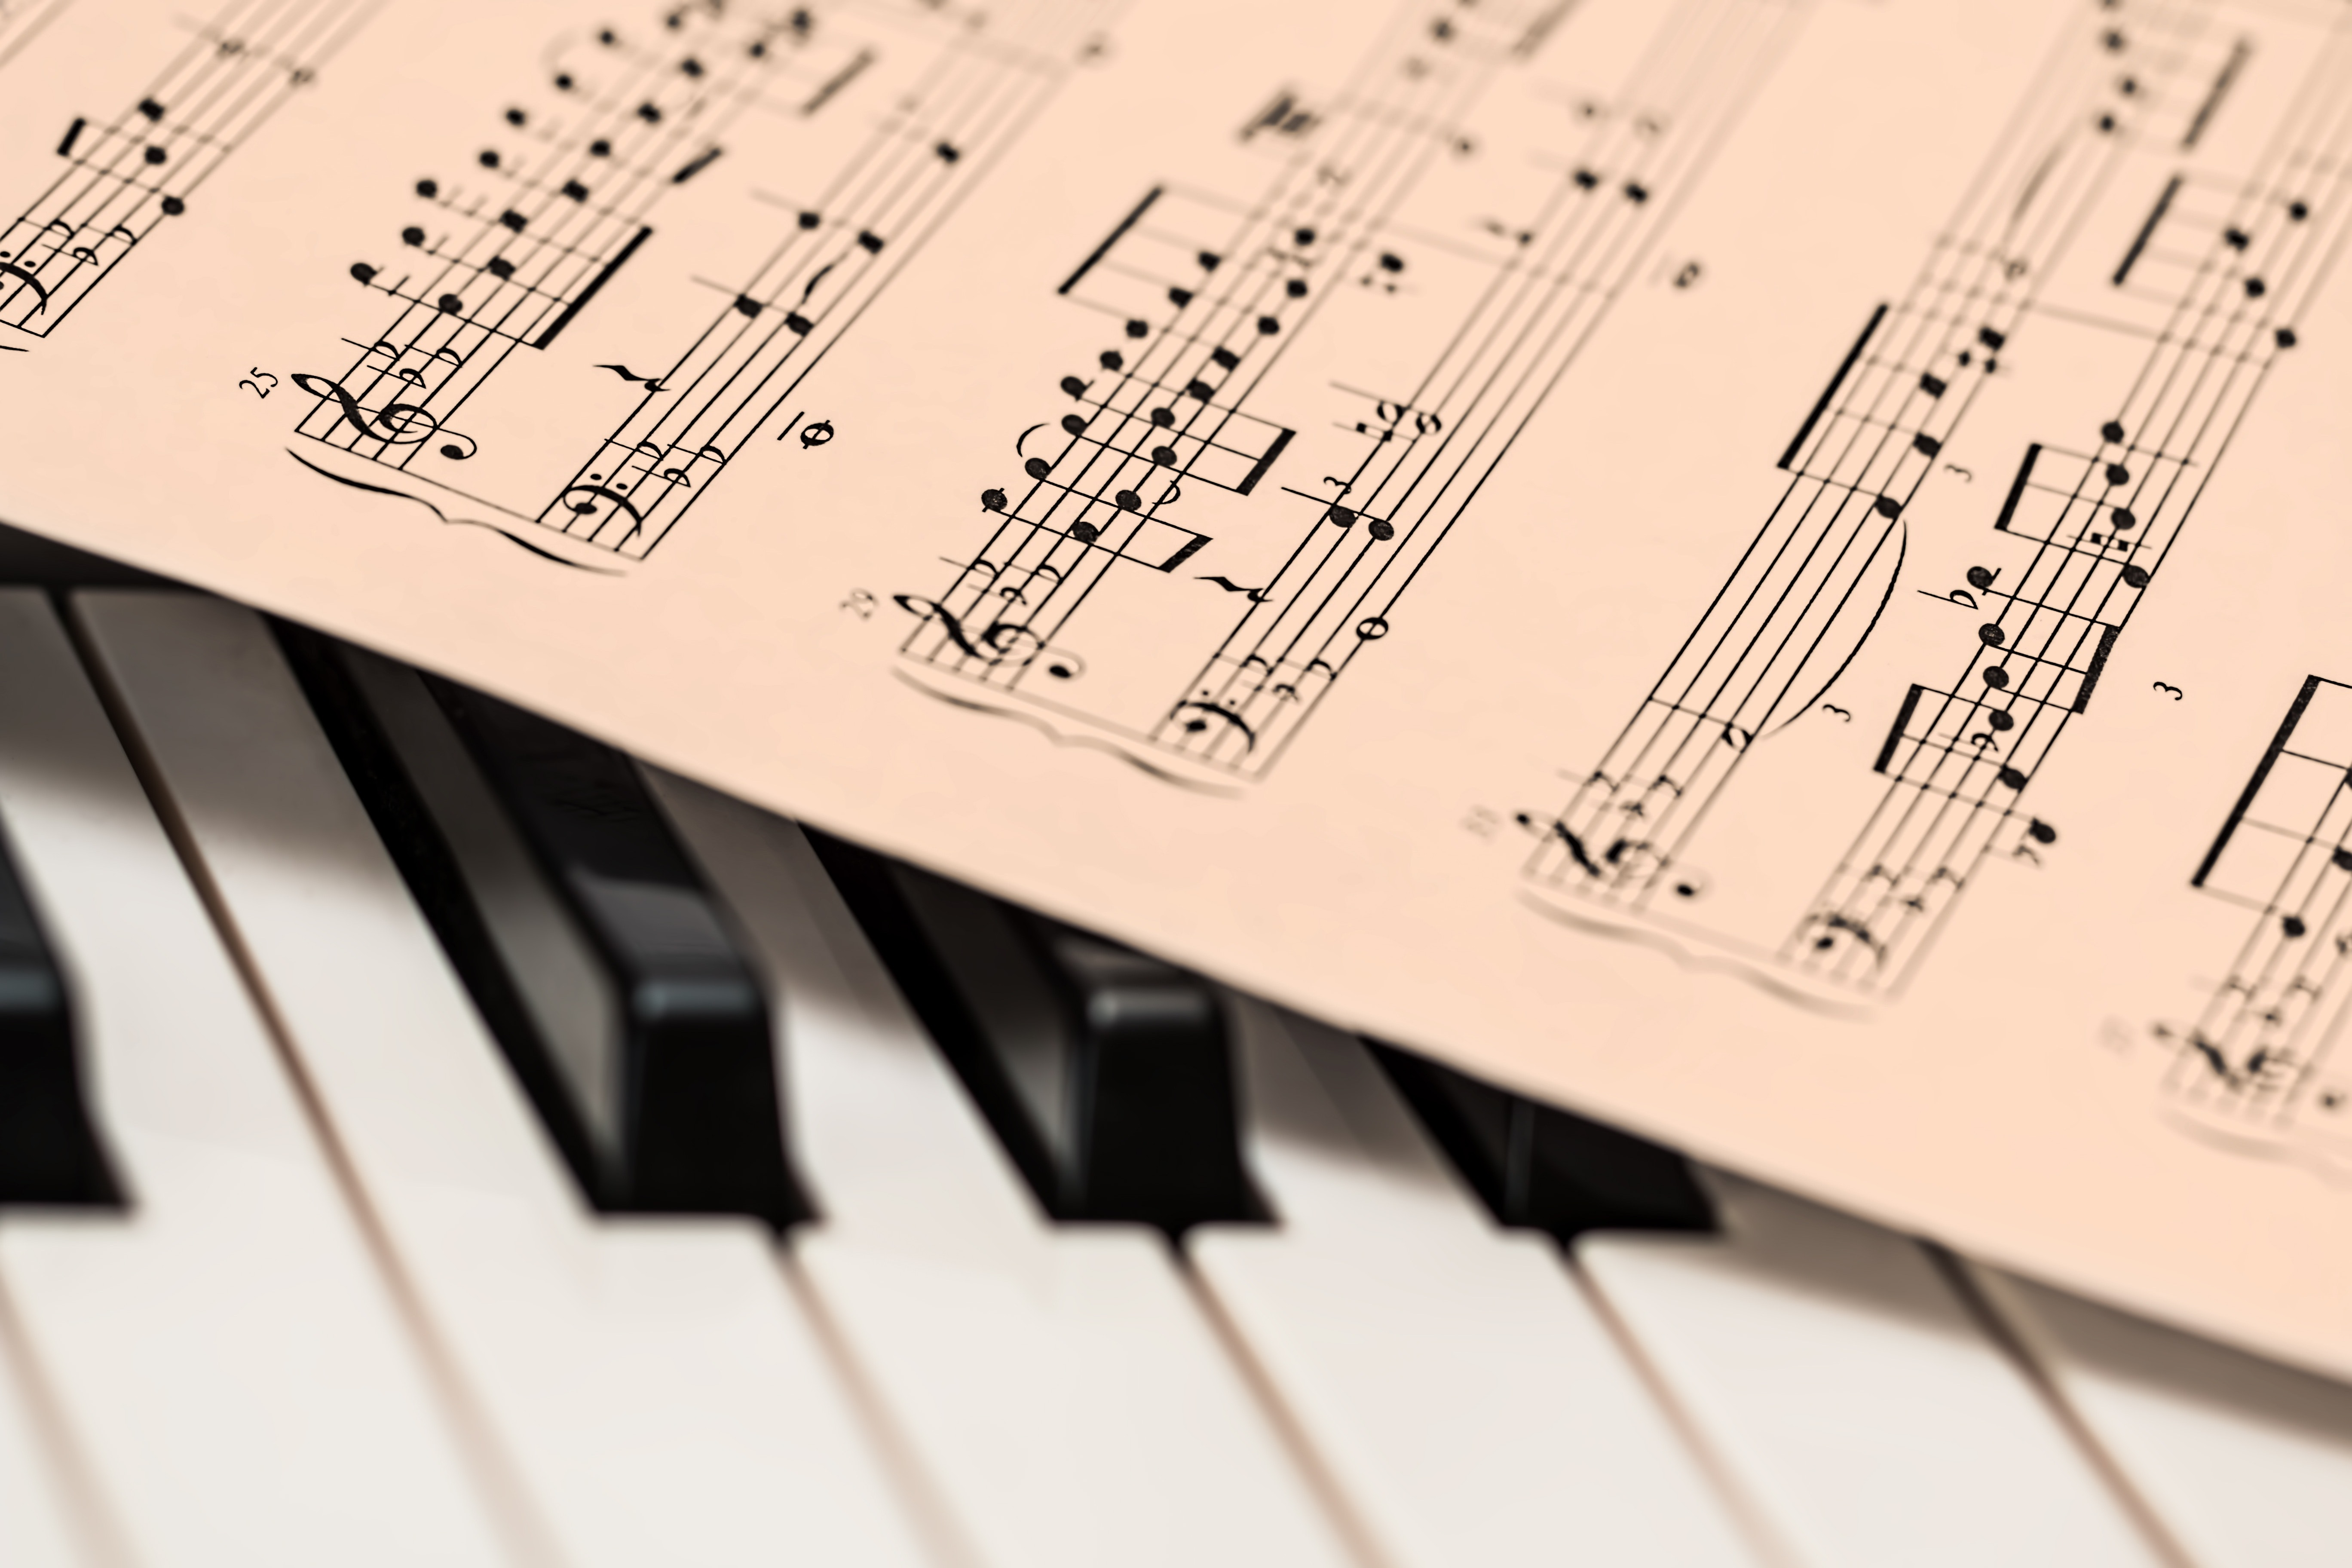
\includegraphics[width=0.6\textwidth]{piano.jpg}
        
            \vspace{3cm}
        
            \textit{Prof. Derek G. Bridge}
        
            \vspace{0.5cm}
        
            \textbf{University College Cork}
        
            \textbf{Final Year Project, BSc. Computer Science}
            
            \textbf{April 2023}
        }
    \end{center}
\end{titlepage}

\chapter*{Abstract}
In this Final Year Project I present the use of Case-based Recommendation in creating music playlists, 
along with providing an implementation of this CBR system and examples of output.
Playlists are sequences of songs arranged in a particular order. Using this information, 
context can be gained from previous playlists in order to build a new playlist from a given seed song or starting list. 
Patterns in previous playlists can be analysed and used to create an enjoyable and coherent listening experience.
This paper mainly makes reference to the paper below \cite{main}. 
Other research and ideas were drawn from \cite{constructive-adaptation} and \cite{cbr-general}.

\chapter*{Declaration of Originality}
In signing this declaration, you are conforming, in writing, that the sub-
mitted work is entirely your own original work, except where clearly at-
tributed otherwise, and that it has not been submitted partly or wholly for
any other educational award.
I hereby declare that:
\begin{itemize}
    \item this is all my own work, unless clearly indicated otherwise, with full and proper accreditation;
    \item with respect to my own work: none of it has been submitted at any educational institution contributing in any way to an educational award;
    \item with respect to another's work: all text, diagrams, code, or ideas, whether verbatim, paraphrased or otherwise modified or adapted, have been duly attributed to the source in a scholarly manner, whether from books, papers, lecture notes or any other student's work, whether published or unpublished, electronically or in print.
\end{itemize}
\large{\textbf{Signed:}} \raisebox{-.2\height}{
\includegraphics[width=150pt]{signature.png}} \\
\large{\textbf{Date:}} 12th April 2023

\tableofcontents


\chapter{Introduction}

\section{Music Listening in the Pre-Industrial Era}
Throughout most of history, the only way for a person to listen to a piece of music was to either attend a live performance,
or perform themselves. While the written recording of music as notation has existed for hundreds of years, the majority of the population 
would not have the education and time to be able to read and reproduce this music, aside from the nobility who would have 
court musicians writing and performing music for them. W.A. Mozart, one of the most well-known composers today, had to travel the courts of Europe 
after leaving Salzburg due to low pay and the desire to compose more freely; he battled with financial insecurity throughout his life.
Turlough O'Carolan was a famous blind harper who traveled across Ireland composing planxties for patrons.

This also generated a rift between the 
organised, written music of the elites with professional performers,
compared to more accessible folk/traditional music of the populace which could be performed solo or by a group, and was passed down by ear.

\section{Early Sound Reproduction}
Attempts to reproduce the sound of music have been attempted and improved as technology has advanced,
beginning with spring-wound machines in which a metal pin strikes a series of raised pitches on a rotating cylinder or disc.
Music boxes are the most well-known, and reproduce a single melody line, though more complex contraptions automatically playing flutes,
violins and keyboard instruments also existed, and player-pianos continue to exist, though less common and usually digitally operated.

The issue with these machines is that they would play exactly as inscribed, and with simplistic musicality. They tended to be large, expensive and limited to few tracks.

\section{19-20\textsuperscript{th} Century Innovations}
With the development of early cylinder-based phonographs, followed by disc-based gramophones, allowed the widespread recording of music to occur.
Gramophone recording would inscribe the sound vibrations onto a master record, from which copies would be printed onto shellac-based, and later polyvinyl-based
discs. These discs were analog recordings of actual artist performances and improved in clarity with advances in materials and recording techniques.
Acoustic recording gave way to electronic with microphones allowing more control and flexibility.
Later on, magnetic tape recording was invented, and while initially only used in studio recording,
eventually allowed for a small, portable and rugged music format to be developed in the form of the cassette,
which started being produced from the 1960s and became more popular into the '70s.

Towards the end of the 20\textsuperscript{th} Century, digital solutions to storing and playing music were explored, with the Compact Disc exploding onto the scene in 1982,
effectively replacing any market share records had remaining, and competing with compact cassettes, replacing them for audio playback in the 2000s.

\section[Music Ownership, Albums and The Computer Age]{Music Ownership, Albums and \\ The Computer Age}
Until the rise of computers and the Internet, the way in which people listened to recorded music was starkly different. One would listen typically hear a song on the radio or live, and,
if they wished to listen to it repeatedly, would visit the record store and purchase a copy of the song on vinyl, cassette, or CD. 
Cassettes also allowed for radio streams to be recorded.

They could also purchase a collection, typically an album on the medium of their choice, which would tend to be better value.
In many styles of music such as pop and rock, collections of pieces or songs would be released together by an artist in albums.
Music albums, initially inspired by photo albums, typically comprise a collection of tracks which tend to cover a theme or idea, and are intended by the artist to be listened sequentially.
Even in other genres, music would be grouped and sold, length depending on the format and album. This allowed for longer uninterrupted listening before the
listener would have to change the disc or cassette manually or with a suitable player.

The practice of ``owning'' your own music would continue to remain popular with many people until the advancement of Internet infrastructure and services.
Apple pioneered the digital sale of music online, allowing songs to be purchased individually, to be played on MP3 players such as the iPod.
This broke with the previous paradigm of selling and playing by the album. People now had the ability to create their own custom collections of songs called playlists.
At this point, most people still consciously which songs to purchase, and gathered their own personal collections on their own.
However, with the rise of Napster and later Spotify, this model of music ownership becamse less popular, as people wished to listen to more music without having
to purchase every single song they wanted to listen to. Apple iTunes also started facilitating streaming, leading us to today, where most stream music 
from a platform such as YouTube, iTunes, or Spotify.

\section[Modern Problems Require Modern Solutions]{Modern Problems Require Modern \\ Solutions}
This rise in music streaming, along with the ability to purchase individual songs for a cheap price, has meant that listening to albums from start to finish
drastically reduced in popularity. Many people listen to playlists or just the individual songs themselves as shown in these surveys
carried out by Deezer\cite{deezer} and MusicBiz\cite{musicbiz}.

A major convenience offered by music streaming providers nowadays is the automatic generation of playlists,
making it easier for users to listen to a variety of music without having to create their own playlists manually.
This is now done using many methods ranging from popularity counts (seen in many services as the ``Hot'' or ``Trending'' pages) to personalised user-user and user-item algorithms,
which take into account previous user listening activity and the preferences of ``similar'' users. Thus the problem: \textit{Which
methods generate the most interesting playlists for users?} In this paper, I explore various ways of generating music playlists, focusing on case-based recommendation.


\chapter{General Implementation Details}

\section{Data}
The data was acquired from Spotify's Million Playlist Dataset.
Processing was done on the dataset running in SQLite.
The data was downloaded from Spotify's servers, structured as a set of JSON files.
This was then converted into an SQLite database to improve lookup performance.
Additional data was queried from Spotify's API.

\section{Tables}
\begin{itemize}
    \item \texttt{tracks} -- specific track info, song name, album name, etc.
    \item \texttt{track\_features} -- generic track features as measured by Spotify such as acousticness, danceability, speechiness etc.
    \item \texttt{artist\_genres} -- artists and their associated genres
    \item \texttt{playlists} -- playlist information
    \item \texttt{playlist\_tracks} -- link between tracks and playlists
    \item \texttt{seq2\_simple} -- all sequences of \(\langle song1, song2 \rangle\), usually aggregated in processing
    \item \texttt{similarities} -- artist similarity rating based on their genres
\end{itemize}

\section{Processing}
The implementations are written in \emph{Python}.
This is due to the large amount of useful libraries available for the language such as \emph{Numpy}, as well as the quick 
writing and readability. 

\section{Output}
All algorithms described in this paper take in an input seed song or starting list of URIs, and output a generated list of track URIs.
\\
\\
\texttt{(spotify:track:1, spotify:track:2,\ldots, spotify:track:\(\lambda\))}

\section{Limitations in Song Output}
Due to the nature of Case-based Recommendation, it can only generate playlists containing songs that are already present in the seed dataset, 
thus limited to songs up to 2017.
This is because it ranks songs rather than a generic set of features, and even an output comprising a list of feature sets would be limited to the dataset
due to the inability of querying Spotify by features.

The similarity-based approach likewise only works for precomputed similarities in the dataset.

\section{Limitations in Personalisation}
Personalising songs and genres based on a Spotify User Profile is possible by preferring user playlists and song features
over generic playlists, it was beyond the scope of this project, requiring user authentication, processing and further development of the demonstration \hyperref[chap:webapp]{web-app}.
User-user recommendation and weighting is also theoretically possible, but would require manual input of other users as Spotify does not have a
public API for getting ``similar users''.


\chapter{Similarity-based Recommendation}
\section{Background}
words

\paragraph{Jaccard Similarity}
This was used to precompute the similarity between different songs based on their attributes. 
This can then be used to create a playlist based purely on track similarity.

\[Sim(\bm{s_1}, \bm{s_2}) = \frac{|\bm{s_1} \cap \bm{s_2}|}{|\bm{s_1} \cup \bm{s_2}|}\]


\chapter{Case-based Learning}
\paragraph{Case-based Recommendation (CBR):}
The approach in which a playlist is generated from a seed song/shorter playlist using sequential patterns 
learned from a dataset of existing playlists.
CBR is a method of recommendation which can be used in contexts in which a meaningful order or sequence to objects is desired or useful.
There can also be a large variety of possible values (such as songs in this case).

\section{Case Base}
A set of playlists may then be filtered to remove meaningless and/or noisy playlists, forming the Case Base.
The playlists are then analysed, using their song order as well as the songs themselves, in order to 
come up with new playlists to generate from an initial seed song.

\section{Retrieval of Playlists}
From this Case Base of playlists \(\mathcal{C}\), two main values are computed for each playlist:
\begin{itemize}
    \item The Attribute Variety: How varied and diverse the playlist is, based on song attributes
    \item The Coherence of the playlist: How relevant the sequences are to the seed song, as well as how many
\end{itemize}

After computing the Variety and Coherence for each playlist \(p\in\mathcal{C}\), a rating function combines both and allows the playlists to be ordered.
\[\rho(p, s) = Var(p) \cdot Coh(p, s), \forall p \in \mathcal{C}\]

\section{Reuse}
After the \(k\) playlists have been ranked, they have to be then converted in some way to form a single playlist of a particular length \(\lambda\). 
This is to be done using a process called Constructive Adaptation(references \cite{constructive-adaptation} in \cite{main}), which comprises of two parts:
\begin{enumerate}
    \item Hypothesis Generation(HG): How partial solutions are extended from the currently generated state of the playlist 
    (either the seed song at the beginning or the highest ranked generated sequence chosen by HO afterwards)
    \item Hypothesis Ordering(HO): Uses the ranking of sequences from \(\mathcal{C}\) to rank the list of newly generated playlists after each iteration of HG
\end{enumerate}
An ideal solution is generated by appending or prepending a song at a time to the seed song, decided but creating potential successor 
solutions using Hypothesis Generation and ranking using Hypothesis Ordering. 
This is continued recursively down the most ideal node. However, if no successor solution is generated at a particular level, then it is discarded from the 
list of ranked generated sequences, and the process continues from that point, until a playlist of length \(\lambda\) is generated.

\section{Formulae Used}\cite[pp. 5--10]{main}
\paragraph{Variety}
The variety of each playlist in \(\mathcal{C}\) is calculated based on the repetition of song features within a set distance. 
This is first calculated per attribute and then each attribute's variety is combined together:
\begin{equation}
V_a(p) = \prod_{i=1}^n
\begin{cases}
    \frac{j-i}{\gamma_a} & \text{if}\ \exists j, i < j <= \min(n, i+\gamma_a) : a(s_i) = a(s_j) \\
    & \wedge\ \forall k, i < k < j, a(s_i) \neq a(s_k) \\
    1 & \text{otherwise}
\end{cases}
\end{equation}

If no value of \(a\) is repeated within the safe distance \(\gamma_a\), then \(V_a(p)\) is 1. Otherwise it is some value between 0 and 1.
Combined variety for all attributes \(a \in \mathcal{A}\) for playlist \(p\):

\[Var(p) = \prod_{a\in\mathcal{A}} V_a(p)\]

\paragraph{Coherence}
The coherence of each playlist in \(\mathcal{C}\) is calculated based on how related it is to the input song. 
In order to calculate the Coherence for each playlist, the Relevance is first computed. 
The Relevance is determined by the amount of times the sequence \(q\) appears in the playlists that make up \(\mathcal{C}\), 
adjusted for the biases of length and song popularity, and returns the degree in which \(q\) is a relevant pattern for song \(t\).
\[Rel(q, t) = \phi(q) \cdot \frac{\alpha^{\theta-\Lambda(q)}}{\psi^\beta(q, t)} \]
The Coherence is then calculated from the sum of all these relevant patterns in a particular playlist.
\[Coh(p, s) = \sum_{q\in\Omega(s, p)} Rel(q, s) \]

\paragraph{Hypothesis Generation}
The nodes generated at each stage are sequences of songs from the \(k\) playlists, and consist of \(T = (t_1, t_2, ..., t_n)\) songs. 
\(T'\) is a successor playlist, thus it contains all \(t \in T\), along with an additional song \(u\). This song is either prepended or appended to the list 
of songs. Thus \(T' = \langle u + T \rangle\ \text{or}\ \langle T + u \rangle\).

Considering the first case, \(u + t_1\) should appear at least once in the set of \(k\) retrieved playlists, in order to be coherent. Similar is done 
in the second case, where \(t_n + u\) should appear at least once in \(k\). Thus the set of all successors would be all combinations of these two rules done recursively.

\paragraph{Hypothesis Ordering}
The sequences are ordered by computing their Relevance and Variance, similar to how the \(k\) playlists were chosen. 
\[H(T') = Rel(T', u) \cdot Var(T')\]
Where \(T'\) is the successor list and \(u\) is the added song. 
However, in order to determine whether future evolutions of \(T'\) will also be varied and coherent, a look-ahead parameter is added.
\begin{itemize}
    \item L = 0: The above formula is applied as is
    \item L = 1: \(H\) is performed on all the successors of \(T'\), and the maximum value found is returned 
    \item L = 2: \(H\) is performed on \emph{all the successors} of all the successors of \(T'\) (depth 2), and the maximum value is returned
\end{itemize}
As with many such parameters, a trade-off between precision and performance has to be chosen, as computing cost increases exponentially with \(L\).



\chapter{Testing}
A variety of CBR systems will be tested with varying weightings of Coherence and Variance, along with the simpler pseudorandom and similarity-based algorithms.
These will then be ranked out of 10 by survey, with top ranked lists passed back into the dataset.



\chapter{Web Application} \label{chap:webapp}
words


\printbibliography

\chapter*{Reference Links}
\normalsize{
\begin{itemize}
    \item Spotify Million Playlist Dataset -- \url{https://engineering.atspotify.com/2018/05/introducing-the-million-playlist-dataset-and-recsys-challenge-2018/}
    \item Spotify Web API Docs -- \url{https://developer.spotify.com/documentation/web-api}
    \\
    \item MusicBrainz -- \url{https://musicbrainz.org/}
    \item Million Song Dataset -- \url{http://millionsongdataset.com/}
    \\
    \item Python Documentation -- \url{https://docs.python.org/3.11/index.html}
    \item SQLite Documentation -- \url{https://www.sqlite.org/doclist.html}
    \item Numpy Documentation -- \url{https://numpy.org/doc/stable/index.html#numpy-docs-mainpage/}
    \item Vue.js Documentation -- \url{https://vuejs.org/guide/introduction.html}
    \item Golang Documentation -- \url{https://go.dev/doc/}
    \\
    \item Sheet Music on Keys Image -- \url{https://www.pexels.com/photo/chords-sheet-on-piano-tiles-210764/}
\end{itemize}
}
\end{document}
